%!TEX program = xelatex
\documentclass[titlepage,11pt,a4paper]{article}
\usepackage{amssymb}
\usepackage{dsfont}
\usepackage{graphicx}
\usepackage[ruled,vlined]{algorithm2e}
\graphicspath{ {results/} }
\usepackage[titlepage]{polytechnique}


\title[INF 431 Programming Project]{Set multijoueurs}
    %\subtitle{Le sous-titre (optionnel, enlever cette ligne sinon)}
    \author{Zuli \textsc{HUANG}\\
            Yunxiang \textsc{ZHANG}
            }
    \date{06/04/2017}

\begin{document}
\maketitle

\section{Application à un joueur}
Dans un premier temps, nous avons développé une application pour un joueur seul sous Android.

\begin{figure}[h]
    \centering
    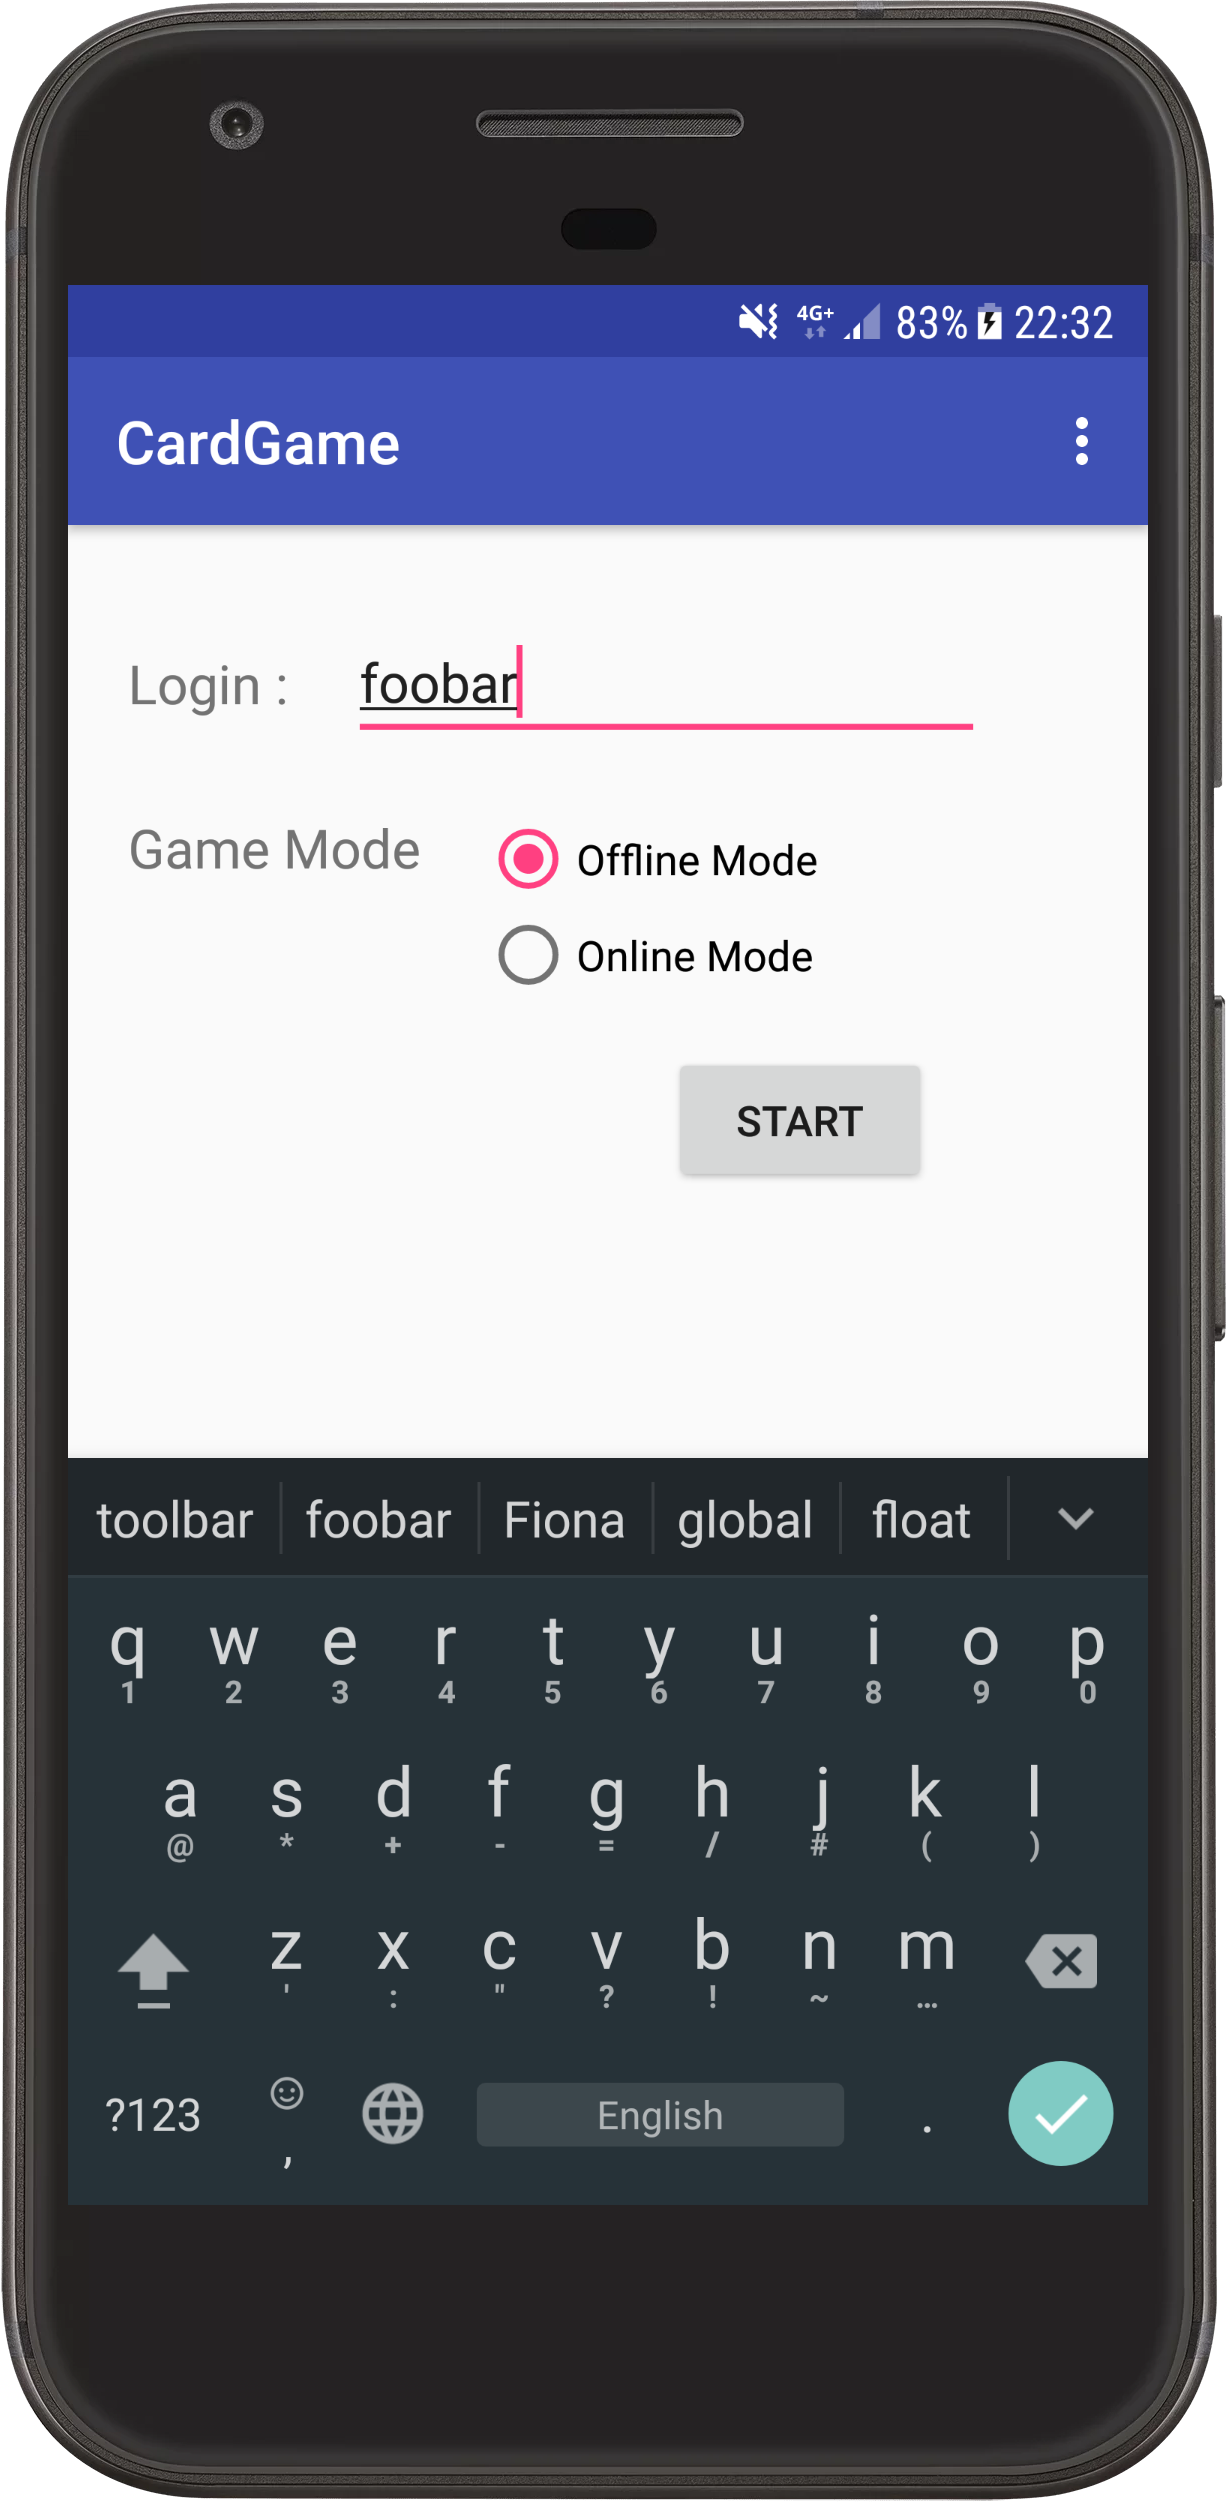
\includegraphics[width=\textwidth]{login_screen.png}
    \caption{Login Screen}
    \label{fig:questioin_1.2_out}
\end{figure}

\end{document}
